% OB-SECTION {"id":"introduction","label":"sec-introduction","level":2,"order":1,"title":"Introduction"}

\section{Introduction}
\label{sec-introduction}
% OB-EDIT-BEGIN openbarry/markdown@1 id=introduction
Diversity of opinion, preference, and experience is a fundamental trait of being human.
If you were to ask ``Tell me a joke'' or ``What is the best book of all time?'' to the next five people you talk to, with high likelihood you would receive five different answers.
It is reasonable to expect language models to generate responses that have the same level of diversity as humans.
Yet, when we ask models such as GPT-4 to recommend a movie or Claude~3 to suggest several vacation destinations, we often receive variations of the same few ideas---a phenomenon known as mode collapse~\cite{hamilton2024}.

\obtodo[id=nb-opening-motivation, created=2024-10-08T18:22:11.000Z, updated=2025-03-21T11:04:33.000Z, completed=2025-03-21T11:04:33.000Z]{Write the opening motivation around jokes, books, and mode collapse.}

This lack of diversity in language model outputs represents a significant limitation.
Today's aligned language models tend to produce lower entropy distributions than earlier generations of models~\cite{zhang2024diffuse}, and when asked to generate (using random sampling) several responses to an open-ended prompt, the responses will often contain substantial near-duplicates~\cite{omahony2024}.
This tendency can harm the utility of these models for subjective tasks where different users may have diverging preferences and needs~\cite{zhang2024diverging}.
Sorensen et al.~\cite{sorensen2024} refer to the inability of today's LLMs to produce diverse generations as a failure of \emph{pluralistic alignment}.

While today's LLMs are evaluated at great length for knowledge and reasoning abilities, they are rarely evaluated for response diversity, and there are no widely-adopted benchmarks for assessing this trait.
The majority of existing evaluation benchmarks are ``mode-seeking'': they only assess the quality of the most likely generation and do not assess the capability of models to produce meaningful alternatives.
In an analysis of 67 benchmark papers published at COLM 2024 and ICLR 2025, we found that over 90\% of these papers evaluate language models based on a single/best generation.

\obtodo[id=nb-colm-iclr-survey, created=2025-01-09T09:15:00.000Z, updated=2025-02-17T16:41:22.000Z, completed=2025-02-17T16:41:22.000Z]{Count single-generation vs distributional eval in COLM 2024 and ICLR 2025 benchmark papers.}
\obcomment[kind=result]{67 papers, over 90 percent single/best generation. Keep this in the intro, it is the incentive argument.}

In this work, we set out to measure not only what language models can generate, but also what they cannot.
We propose \textsc{NoveltyBench} (Figure~\ref{fig:overview}), a benchmark for measuring how well language models can generate multiple differing but still correct answers to user requests that involve subjectivity, randomness, and creativity.

\begin{figure}[t]
\centering
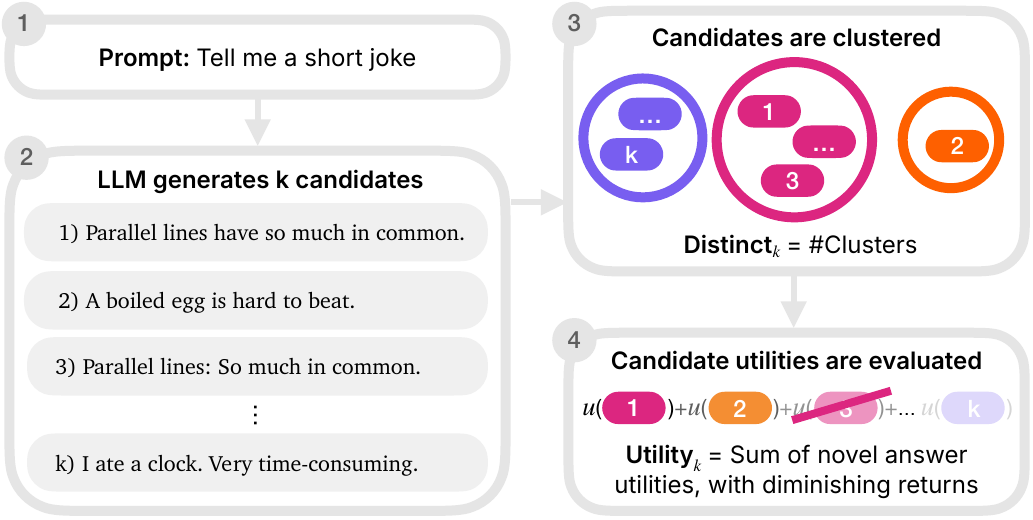
\includegraphics[width=0.95\linewidth]{figures/eval_figure_1.png}
\caption{\textsc{NoveltyBench} overview.
We partition generations into functional equivalence classes and introduce two metrics: $\mathrm{distinct}_k$ counts unique equivalence classes among $k$ samples, and $\mathrm{utility}_k$ combines novelty and quality, weighing utility of individual generations by user patience ($p=0.8$) and only considering novel generations.}
\label{fig:overview}
\end{figure}

In summary, we introduce \textsc{NoveltyBench}, a benchmark consisting of 1,100 prompts that we expect to elicit variable answers from humans, 100 of which are annotated with responses from eight human annotators.
We propose a unified measure of novelty and quality which can be used to gauge how well an LLM can produce diverse, high-quality responses to a given prompt.
We evaluate \textsc{NoveltyBench} on twenty frontier models, including GPT-4o, Claude 3.5 Sonnet and Gemini 2.0 Pro, and find that all suffer from a lack of diversity.
Our evaluation further reveals that larger and more capable models in the same model family tend to produce less diverse outputs.

\obclaim{State-of-the-art models generate significantly less diversity than humans, producing on average fewer than 4 distinct responses in 10 samples, and novelty scales inversely with model size within a family.}
% OB-EDIT-END id=introduction
